\documentclass[11pt, a5paper, twoside]{book}

\usepackage{float} % incluir imagens
\usepackage[export]{adjustbox} % centralizar
\usepackage{subcaption} % legendas
\usepackage{graphicx}
\graphicspath{ {pic/} }

\usepackage[pass]{geometry}

\usepackage{setspace}
\setstretch{1.2}

\usepackage{indentfirst}
\usepackage[skip=0pt, indent=1.25cm]{parskip}

\usepackage{ragged2e}
\justifying{}

\usepackage[portuguese]{babel}
\usepackage{hyphsubst}

\usepackage{fontspec}
\usepackage{hyphenat}
\hyphenation{pre-pa-ra-va=me}

\newenvironment{dedication}{
    \clearpage
    \thispagestyle{empty}
    \vspace*{\stretch{3}}
    \small
    \itshape
    \raggedleft
}{\par\vspace*{\stretch{1}}\clearpage\normalfont\justifying} % taken from https://tex.stackexchange.com/questions/476646/how-put-title-in-a-dedication

\title{História da Família, Parte II}
\author{Teresa Cristina}
\date{2025}

\renewcommand{\thechapter}{\Roman{chapter}}

\addto\captionsportuguese{
    \renewcommand{\contentsname}{Sumário}
}

\begin{document}

\begin{titlepage}
\maketitle 
\end{titlepage}


\begin{dedication}
Aos meus filhos, para que, tal como ensinou Terêncio, nada que seja humano, seja-lhes estranho. 

Aos que cobrarem maior fidelidade aos fatos, saibam que o que aqui vai contado, vai tal e qual a emoção esculpiu na alma e a memória arquivou sem contestar. 
Pois nunca sabemos com exatidão o que de fato acontece. 
O que fica é o que nos parece e como nos parece no momento do acontecido. 
\end{dedication}

\tableofcontents

\chapter{}
Sou do tempo bom em que os adultos se livravam das crianças sem culpa, mandando: ``Vão brincar lá fora!''.
E ``lá fora'' era o quintal, o maravilhoso país da infância.
Sobretudo quando se vivia numa cidade do interior. 
Era o espaço de descobrir e pensar o mundo. 
Observar as formigas na sua labuta incessante, as lagartixas subindo pelo velho muro meio rachado, as borboletas iridescentes, o rastro prateado e gosmento desenhado pelos vagarosos caracóis.   
Contemplar a incessante migração das nuvens que o vento ora esfiapava, ora ia juntando em formas caprichosas de bichos, árvores, gigantes, castelos, anjos e às vezes mapas, como aqueles pendurados nas paredes da sala de aula. 
Sentir o cheiro da roupa lavada e embebida de sol, pendurada no varal; da fumaça desprendendo-se da lenha queimada no fogão; da terra molhada, da moita de arruda, das rosas, do jasmim, do manacá; do bafio úmido de sepulcro que emanava da escura caverna do porão. 
Deitada de costas nas pedras quentes da calçada, abandonava-me ao sol. O calor invadia aos poucos meu corpo, amolecendo braços e pernas e eu os imaginava penetrando terra adentro, como raízes. 
Imóvel, escutava o zunido das abelhas nas flores, os recados insistentes do ``fogo apagou'' e do bem-te-vi vindos lá das bandas do cemitério, o canto dos sabiás e a algazarra dos pardais e andorinhas sobrevoando a velha paineira do almoxarifado da prefeitura bem ali, do outro lado da rua. 
Na marcenaria, alguns quarteirões acima, o som plangente da serra cortando madeira dividia com o sino da torre da Matriz a tarefa de marcar regularmente a passagem das horas. 
Vez ou outra, roncando em agonia a cada mudança de marcha, os velhos ônibus a querosene passavam sacolejando nos paralelepípedos, rua acima; os carros ainda eram raros. 
E, do outro lado do muro, do barracão da fábrica do meu pai, chegava o som oceânico, abafado e constante das máquinas torcendo os fios de algodão para transformá-los nos novelos de barbante que garantiam o sustento da nossa família e a minha doce vadiagem de criança.

As cores, formas e textura das flores e folhagens me fascinavam. 
Recobriam meus desenhos infantis e emolduravam em cercaduras delirantes as páginas dos meus cadernos de escola.

Na opinião da minha mãe, as flores do nosso quintal deviam obedecer à moda, como tudo o mais. 
Lembro-me da fase dos crisântemos, dálias e crisandálias repolhudas, logo repudiadas em favor das rosas que, por sua vez, acabaram arrancadas para dar lugar às palmas de Santa Rita e às gérberas. 
Essas mudanças eram quase sempre decididas por volta do Dia de Finados, quando as parentes da Capital chegavam sobraçando as novidades compradas nas floriculturas do Arouche. 
Houve uma vez em que a matriarca das hostes paulistanas, Tia Angelina, desceu do trem exibindo buquês de soberbos e inacreditáveis gladíolos azuis. Foi o quanto bastou para que as nossas pobres palmas de Santa Rita caíssem em desgraça. 
``Coisa mais calú!'', decretou minha mãe. 
Era sua expressão favorita para o que lhe parecia vulgar ou caipira. O projeto do novo jardim teve, porém, que ser adiado. 
De tanto mexer na terra, nas sucessivas reformas dos nossos canteiros, mamãe arrumou uma infecção persistente nos dedos que acabou por lhe fazer caírem as unhas. 
Até um médico especialista em São Paulo precisou ser consultado, já que o nosso habitual curandeiro, o Joãozinho da Farmácia, amigo de longa data do papai, não conseguiu resolver a tal eczema.

De qualquer modo, outros e mais amplos planos de mudança começavam a agitar minha família, pois mamãe começara a achar ``calús'' não só as flores, como todo o quintal, a casa antiga de ``parede a meia'' e banheiro fora, os móveis escuros, ``art-déco''. 
Papai prosperava nos negócios e mamãe já podia sonhar mais alto: uma casa moderna, com mais cômodos, armários embutidos, num bairro novo e mais nobre. 
Prenunciando a nova fase, nossa antiga sala de jantar desapareceu para dar lugar a uma mobília nova e aromática, de jacarandá torneado, em que se destacava uma vistosa cristaleira apropriadamente recheada com copos de cristal recém-adquiridos e que tilintavam perigosamente a cada passo nosso sobre o velho assoalho. 
Nossas caminhas \textit{Patente} foram substituídas por outras, artisticamente torneadas também e os velhos colchões de crina foram para o lixo. 
Passamos a dormir em modernos colchões de mola. Um tapeceiro alemão veio tirar as medidas para fabricar sofá, poltrona e cortinas para a sala de estar. 
Coroando todo esse luxo, um dia desembarcou em nosso portão a peça central da nova decoração: um piano de nogueira, novo em folha, que se converteria num dos grandes instrumentos de tortura da minha juventude. 
Porque então, junto com o quintal e a velha casa, ficava para trás também a minha infância. 
Eu me tornara uma adolescente e, em breve, nós mudaríamos para a casa da Av. D. Pedro II, n.º 1273, defronte ao Clube de Campo do Araraquarense. Corria o ano de 1958.

\begin{figure}[H]
\centering
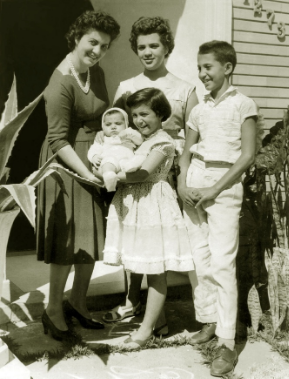
\includegraphics[width=0.5\linewidth]{1/maria-joão.png}
\caption{A família na porta da casa nova. No colo da
Maria Lúcia, o recém-chegado João.}
\end{figure}
\chapter{}
Para o bem e para o mal, minha infância transcorreu numa pequena galáxia de clãs interligados, de origem imigrante e pobre, dos quais os mais importantes eram os Filpi, os Credidio e os Ópice, todos com raízes na Itália. 
Dezenas de olhos e bocas para censurar e orientar e montes de braços para acarinhar e acolher, e uma intensa experiência humana para vivenciar, recolher, degustar e aprender. 

Nossa antiga sala de jantar exibia uma mesa particularmente desgraciosa, quadradona e pesada, mas que, para mim, tinha um encanto especial: embutia um pequeno armário no seu único e largo pé central, onde eram guardados os jornais velhos. 
Um dia descobri que eu cabia direitinho naquele esconderijo e ali, insuspeitada, colhi minhas primeiras e fortes impressões do mundo adulto.  
Era à volta daquela mesa que as visitas se reuniam para o café. 
Era divertido acompanhar, debaixo dela, o movimento das pernas inchadas e nodosas de varizes das tias-avós, na excitação de comentar os acontecimentos da cidade e a vida alheia. 
Quando mamãe e suas irmãs aparteavam a discussão, vez ou outra, contrapondo argumentos mais modernos, arejados por visões do pós-guerra de liberação feminina, difundidas pelo cinema norte-americano quase sempre, as vozes se alteravam, os pés se agitavam e, na ânsia de vencer a contenda, de algum ponto da mesa vinha a cartada definitiva, o disse-me-disse mais recente e irretorquível, quase sempre sussurrado, inalcançável à minha parca compreensão de criança, mas emoldurado pela aura sagrada e misteriosa do interdito\dots 
Um \textit{``oooohhhh!''} seguido de horrorizado silêncio parecia encerrar a conversa. 
Que logo, porém, renascia animada, como fogo sob as cinzas, sempre sublinhada embaixo da mesa pelo entusiasmado balé de pernas e pés. 
Lembro, com nitidez, de uma tarde em que, andando com minha mãe pela rua, ouvi-a chamar a atenção de uma amiga para uma célebre senhora, personagem recorrente nas reuniões à volta da tal mesa, pelo que me lembro, pelas audaciosas e repetidas incursões fora da sagrada cidadela do casamento. 
Olhei na direção indicada e vi uma mulher vestida de preto, grave e majestosa, na penumbra do banco traseiro de um carro escuro e grande.
Divisei-lhe as feições, ainda bonitas na maturidade. 
Séria, ela devolveu o meu olhar fascinado. E o que senti, juro, foi pura admiração.

Dos clãs principais, o da minha mãe era o mais pobre. 
Incluía as irmãs da minha avó Didi, seus maridos e filhos. 
Meu avô João já não tinha mais parentes próximos. 
Dele só conheci um primo engraçado, que vez ou outra aparecia e de novo sumia, como um cometa.  
Embora todas fossem casadas, as Credidio, mulheres invariavelmente fortes e batalhadoras, sobrepunham-se aos machos em autoridade. 
Dessa gente me vieram os impulsos de amar a vida, de superar os revezes sem esmorecer, de correr atrás dos sonhos, mas também a preocupação com as aparências alimentada pelo receio permanente de incorrer em vulgaridade e mau-gosto. 
Alimentavam ambições sociais e acreditavam piamente em cultivar as boas relações para vencer as desvantagens da origem humilde.  
No riso e no pranto, eram pau para toda obra. Com a mesma disposição para encarar bailes e velórios, casamentos, batizados e procissões, envolviam-se em tudo com igual disposição de fazer todo o necessário para que tudo saísse perfeito. 
Davam-se a todas essas empreitadas com sincera devoção e autêntico espírito de caridade e solidariedade. Mas, não dispensavam os holofotes e tinham a deliciosa ingenuidade de nem tentar disfarçar o prazer que sentiam com a repercussão favorável.

O clã do meu pai, os Filpi, embora menos pobre na sua origem, na Itália, já conhecia há muito a inconstância dos fados. 
Lá, na pequena Novi Velia, o patriarca Ângelo viu seus bens esvaírem-se no torvelinho das brigas políticas. 
Aqui, seu filho e meu avô Reginaldo, fazendeiro abastado a quem o café proporcionara razoável fortuna, casa confortável na cidade e educação de qualidade para a prole, perdeu quase tudo na crise de 1929 e teve que levar a família de volta ao recomeço duríssimo na Pedra Branca, única fazenda que lhe restou das quatro ou cinco que chegou a possuir. 
Por conta desses reveses, com certeza, dessa gente me veio um realismo prudente, alicerçado na crença de que estamos cá na terra a serviço e não a passeio, na desconfiança de que todo ídolo oculta pés de barro e de que tudo que reluz quase nunca é ouro, além do mau hábito de trabalhar até o limite das forças. 

O reino das mulheres Filpi era o lar. 
Exímias cozinheiras, incansáveis no lavar, passar, esfregar, bordar e tecer, foram condenadas à vida espartana pelo atraso da minha avó Teresa, uma mente forjada pelo rígido código dos antigos costumes mineiros. 
Mulher era para servir ao homem, pai, irmão ou marido e não para bater pernas na rua e perder-se como as moças pintadas, ataviadas e oferecidas que se viam por aí, querendo diploma, frequentando bailes, usando saias curtas, dirigindo e até fumando! Quando minha mãe, professora formada, frequentadora contumaz dos bailes do clube, exibindo impecáveis unhas esmaltadas e envergando trajes e penteado da moda ingressou na família, não fosse o apoio imediato do galante sogro Reginaldo, certamente seria rechaçada como péssimo exemplo. 
E pelo resto da vida, mesmo após a morte da Vó Teresa, a relação da minha mãe com as cunhadas, foi contraditória: Lectícia era o farol que iluminava para elas os difíceis caminhos da inserção social e da modernidade. 
Mas mamãe, por muitos e muitos anos, padeceu da necessidade neurótica de provar que, apesar das unhas feitas e das roupas da moda, era páreo para elas no comando de um fogão, de um ferro de passar e no brilho das panelas. 
Daí por que preparar um almoço para as cunhadas era um feito precedido por dias de insuportável e cômica tensão, mas que valiam pelo gosto insuperável da vitória, quando o molho e a massa se apresentavam indiscutivelmente no ponto certo. 
Por outro lado, as tias, com meu ouvido treinado em escutar conversa de adultos, ouvia-as muitas vezes lamentar o destino do irmão, coitado, condenado a trabalhar para sustentar os luxos ``daquela gastadeira''.

Os Ópice eram oriundos do casamento de duas irmãs da minha avó materna com dois irmãos recém-chegados da Itália e que vieram estabelecer-se em Araraquara: um hábil alfaiate, chamado Bruno e um não menos hábil carpinteiro chamado José. 
Ao que se conta, ambos exibiam como característica principal um certo refinamento de gostos, incomum entre os pobres imigrantes italianos da região e que provavelmente lhes pareceu suficiente para justificar uma postura algo arrogante e prepotente que sempre os distinguiu, tanto quanto os rompantes de temperamento. 
Afora isso, eram muito trabalhadores e competentes. Todos esses traços são ainda bem visíveis na sua descendência. 
O ramo do Tio Bruno, quase todo, enraizou-se em definitivo na cidade e o do Tio José, algum tempo após a morte precoce deste, acabou migrando para a Capital. 
Os filhos do Tio Bruno, que continuaram a viver sob o jugo do pai, jamais amadureceram totalmente e ficaram na minha memória como uma família de gente boa, meio infantilizada e divertida. 
Os órfãos do Tio José, libertos do autoritarismo paterno, com muito mérito e muito trabalho, fizeram carreira e sólida fortuna na capital. 
E foi assim que se transformaram, para toda a gente da minha mãe, na referência suprema do sucesso, do ``savoir faire'', o exemplo a ser seguido, fonte de jurisprudência a ser consultada em qualquer circunstância e para qualquer assunto. 
Eram respeitosamente designados como ``os de São Paulo'' e sempre que vinham em visita aos parentes da província provocavam um alvoroço que, à medida que nós, os mais novos, crescíamos, acabou virando motivo de piadas sempre recebidas como sacrilégio por vovó, mamãe e suas irmãs. 
Já meu pai que, como bom Filpi, nunca foi afeito a idolatrias de qualquer espécie, fechava o tempo e não foram poucas as vezes em que os pobres Ópice acabaram pagando pela admiração incompreensivelmente servil, no entender do marido, que minha mãe devotava às ideias e realizações dos primos.
\chapter{}
Em meados do século XX, o castigo físico para a meninada não só continuava em pleno vigor, como em doses razoáveis era considerado instrumento eficiente na construção do caráter infantil. 
Já não se usava a palmatória nas escolas, mas ``a régua cantava'' regularmente nas salas de aula sem que alunos ou pais pensassem em recorrer à justiça por causa disso. 
Era até de bom-tom, como testemunho de confiança e parceria, que estes últimos, ao entregar seus filhos aos mestres, delegassem a eles a prerrogativa de puxar-lhes as orelhas sempre que necessário.

Herança do meu avô Reginaldo, na minha casa havia um \textit{rabo-de-tatu}, uma espécie de chicote feito com pouco mais de três palmos de couro de sola, grosso, arrematado por um cabo trançado em torno de uma argola de metal pela qual ficava pendurado atrás da porta da cozinha. 
Originalmente, tal instrumento era usado para espicaçar a montaria. Como meu avô era exímio cavaleiro e vivia de chicote em punho, deve ter sido só uma questão de oportunidade para que o artefato se convertesse em recurso pedagógico. 
Por sorte, na maioria das vezes, o rabo de tatu da minha casa servia mais à intimidação do que ao uso propriamente dito. 
As surras ``para valer'' eram ministradas sempre pelo meu pai que, explosivo como era, preferia usar suas temíveis manoplas ao invés de perder tempo indo atrás do tal relho. 
Minha mãe é que às vezes o usava para potencializar a escassa força dos seus punhos femininos. Mas, na maior parte do tempo ela recorria apenas aos beliscões, aos tapas e às ameaças:

{\itshape “ -- Deixa estar! Vou contar tudo ao seu pai quando ele chegar e aí eu quero ver!”}

Essa história de apanhar me parecia revoltante pelo que atentava contra a dignidade das pessoas. 
Sentia-o mesmo quando muito menina para sabê-lo. 
Minha mãe apenas me irritava quando me batia, mas com meu pai era diferente.  
Principalmente porque eu tinha uma forma peculiar de reagir ao medo e que redundava numa humilhação ainda maior: eu me urinava todinha, só de pressentir a iminência do seu ataque de cólera. 
Bastava que ele entrasse porta adentro me chamando e escandindo as sílabas do meu nome, anúncio inequívoco das bofetadas que viriam. 
As pernas amoleciam e eu me agachava, passiva, em meio à poça que se alastrava em torno de mim. Com o tempo, percebi que o meu terror parecia aplacar-lhe a ira. 
Eu acabava apanhando menos que meu pobre irmão que, rebelde, usava toda a agilidade das suas magras perninhas para fugir, certo de que papai, pesado e lento, jamais conseguiria alcançá-lo. 
Mas a estratégia se revelava pior. Mais enfurecido, quando lhe punha as mãos, meu pai parecia perder a noção da absurda desproporção entre o seu tamanho e o da frágil criança. 
Mais de uma vez circunstantes assustados intervieram com medo de que ele arrebentasse o menino. 

Apanhamos com alguma constância, meu irmão e eu até a adolescência. 
Não porque evidenciássemos uma inclinação acentuada para a delinqüência. 
Ao contrário. 
Éramos bons alunos e nosso repertório de travessuras nunca excedeu o limite do esperado numa época em que as crianças “eram para ser vistas, mas não ouvidas”. 
Reginaldo era um garoto vivo e muito esperto. 
Foi sempre festejado por essas características e, até onde me lembro, meus pais pareciam orgulhosos em ressaltá-las sempre que se referiam ao filho. 
Apanhar por causa disso devia causar uma grande confusão na cabeça dele. Já eu, que Vó Didi chamava de “minha pata-choca”, precisava de uma razão muito forte para sair da minha habitual bonomia. 
Também não conseguia entender o porquê das surras.

\begin{figure}[H]
\centering
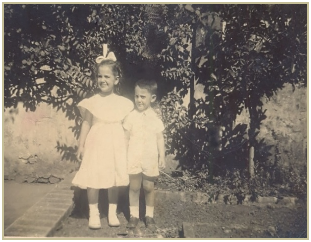
\includegraphics[width = 0.9\linewidth]{3/Reginaldo.png}
\caption{Reginaldo e eu por volta de 1950.}
\end{figure}

Uma das primeiras grandes sovas que levei, lembro, foi no Jardim da Infância porque havia, na escola, a atribuição semanal de uma “Medalha de Disciplina” aos que demonstravam melhor comportamento ao longo da semana e num sábado, excepcionalmente, eu não a trouxe para casa. 
Minha professora me deixara tomando conta dos meus vinte e poucos coleguinhas para dar uma escapadela, sabe-se lá para onde e um deles me pediu que deixasse a turma escrever na lousa. 
Com o discernimento a mim conferido pelos meus seis anos, achei que aquela seria uma boa forma de mantê-los ocupados. 
Não foi. 
Quando a professora retornou, havia giz para todo lado e um realizado e barulhento grupo de pirralhos tinha transformado não só a lousa como todas as paredes da sala numa exposição surrealista, sem que eu, impotente, conseguisse contê-los. 
Meu pai nem quis ouvir a história. 
Ainda hoje acho que a professora, D. Lídia, é que devia ter apanhado em meu lugar. 
 
Na família da minha mãe esse tratamento não existia. 
A menos que se levasse em consideração os beliscões e alfinetadas que marcavam os momentos relevantes dos sermões da Vó Didi às filhas adolescentes, enquanto lhes experimentava as costuras. 
Mamãe achava que ela reservava esse momento de propósito para os corretivos. O
Vô João, ao contrário, não só jamais se agastava como se apressava em protegê-las das tempestades maternas. 

Já na família do meu pai, o emprego da força física para dirimir questões de qualquer natureza era um valor muito apreciado. 
Vó Teresa, contava minha mãe, jactava-se de que seus filhos eram homens de resolver qualquer parada “com um soco só”. 

Um fato lembrado com divertida alacridade pelos irmãos Filpi, e exemplo amplamente divulgado do que acabo de relatar, dizia respeito a uma façanha perpetrada por um deles, o Tio Bepe, um rotundo peso-pesado de cento e trinta quilos, quando desconfiou que Tia Antonieta e Tia Glória, suas irmãs e noivas de dois irmãos, proprietários de uma vidraçaria, estavam sendo iludidas. 
Como a data do casamento ia sendo prorrogada ``ad infinitum'' pela família dos rapazes, ele decidiu tomar satisfação com os infelizes vidraceiros que, pálidos de terror, mal conseguiram entender o motivo da intempestiva visita, comunicado aos berros por cima do crepitar dos vidros pulverizados a murros por aquele búfalo ensandecido. 
Nem é preciso acrescentar que, com o estabelecimento, veio abaixo também o sonho das pobres moças de um dia se casarem. 

O castigo físico como recurso educativo era praticado com naturalidade e frequência entre os Filpi. 
Ouvi minhas tias aludirem, mais de uma vez, a uma bizarra norma pela qual, em crianças, quando um cometia uma falta passível de castigo, todos apanhavam para que um não caçoasse do outro. 
E papai lembrava com muito ressentimento uma passagem em que, muito pequeno ainda, distraíra-se observando formigas, deitado de bruços, espichado ao sol, ao invés de varrer o terreiro de café como lhe tinha sido ordenado.  
Sem dizer água vai, o avô Reginaldo, lá da varanda, fez estalar o comprido látego de conduzir charrete e desenhou-lhe um vergão em brasas ao comprido das costas. 
Revoltou-o demais o gesto tão violento quanto traiçoeiro. 
O que não o impediu de, ao crescer, acrescentar sua própria contribuição ao longo prontuário de brutalidades dos Filpi. 
Vovó Teresa nada ficava a dever ao marido no que diz respeito ao emprego da força como recurso disciplinar. 
Ao contrário, dado que Vovô se ausentava com freqüência, na maioria das vezes era a ela que cabia exemplar a numerosa prole. 
Mamãe contava ter presenciado uma cena em que tia Antonieta, a que mais ansiava por uma história de vida diferente daquela que levava em regime de semi-clausura, foi pedir à mãe permissão para continuar os estudos. 
Em resposta, recebeu tamanho safanão que perdeu o fôlego e a fala por longos e angustiantes segundos. 
E ela já era uma mocinha, a coitada.

Não é de admirar que os irmãos Filpi, incluídas aí as mulheres, uma vez adultos, fossem estimados e respeitados pelas numerosas qualidades de diligência, honestidade, generosidade, disponibilidade para com as necessidades do outro, mas igualmente temidos pela fúria demolidora que lhes podia brotar das entranhas quando enraivecidos.  
Naquele tempo, porém, no que toca aos machos da família, esta característica não chegava a causar grande escândalo porque encontrava certo amparo na mentalidade que predominava, como ainda predomina em alguns rincões da nossa sociedade, de que só pelo uso da força bruta um homem se legitima como tal. 
E o público feminino, não se pode negar, só recentemente começou a limitar seu entusiasmo por esse gênero de exibição. 
Mais de uma vez surpreendi uma expressão de orgulho na fisionomia da minha mãe quando meu pai se impunha pela força dos seus músculos. 
E ele nem precisava disso. 
Tinha estatura moral mais do que suficiente para conquistar naturalmente a admiração e o respeito de quantos o conheceram, inclusive e principalmente nossos, dos seus filhos. 

De qualquer maneira, no caso do meu pai, pelo menos, tenho certeza de que a necessidade de afirmar sua autoridade por esse meio era uma das injunções que o atormentavam. 
Tanto que, após cada um desses surtos de raiva primitiva e indomável, ele parecia consumir-se em arrependimento e buscava por todos os modos uma maneira de compensar a vítima: um presente, um passeio, um agrado qualquer. 
Mas jamais conseguiu reagir de outra maneira a uma situação em que se sentisse desafiado.

\begin{figure}[H]
\centering
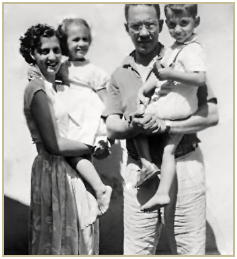
\includegraphics[width = 0.5\linewidth]{3/Familia.png}
\caption{Nossa família, no início dos anos 50.}
\end{figure}

Todos sabem que é contra o muro sólido do poder adulto que os jovens afiam seus dentes e garras. 
Seria preciso que meu pai fosse uma personalidade emocionalmente mais segura para suportar as investidas ditadas pela nossa imaturidade. 
Assombrava-o a possibilidade de cometer erros ou perder as rédeas na condução da família e na educação dos filhos. 
Porque, em nosso meio, esse seria o pior dos fracassos, o mais imperdoável, social ou pessoalmente falando. 
Ao contrário do que se ouve muitas vezes hoje, era opinião corrente que um filho desencaminhado expunha ao mundo a incompetência dos pais. 
Então, naquele tempo, mais que hoje em dia, à medida que a gente evoluía previsivelmente na direção da independência, os problemas em casa tendiam a aumentar na mesma proporção e o chamado “choque de gerações” sobrevinha com impacto terrível sobre as relações familiares. 
De alguma maneira, traumas a parte, esse conflito acabava por exercer uma força centrífuga de tal monta que raras vezes um jovem, depois de experimentá-la, desejava voltar para casa, a não ser depois que achasse um rumo na vida, ou seja, um diploma, um trabalho e até um casamento meio engatilhado. 
Essa podia não ser a forma mais adequada de pais promoverem a autonomia dos filhos, mas funcionava, sem sombra de dúvida. 
Os raros homens ou mulheres que permaneciam em casa, na dependência dos pais, além dos vinte e poucos anos, eram considerados indivíduos frustrados no seu desenvolvimento e olhados com um misto de piedade e estranheza.
As pessoas se perguntavam o que podia ter dado errado.  

Pode-se entender, neste contexto, a insegurança e as reações do meu pai, tendo sido ele próprio, além de tudo, um adolescente um tanto desajustado, sensível e difícil, que por pouco “não se perdeu por aí”, segundo contavam seus irmãos. 
Nele, como me acostumei a dizer, a rebeldia corcoveou até o fim sob a sela pesada da responsabilidade de homem de negócios e chefe de família. 
A repressão violenta exercida sobre nós, sobretudo os seus filhos mais velhos, hoje eu acredito, era também resultado de um esforço hercúleo para exorcizar sua própria inconformidade.

Aos catorze anos decidi que bastava. 
Quando num acesso de fúria meu pai levantou a mão para mim, encarei-o decidida a me defender, fosse como fosse. 
Acho que ele percebeu. Nunca mais repetiu o gesto. 
Paradoxalmente, entretanto, aquela manzorra pesada que tanto me apavorava quando se precipitava como aríete na minha direção, ficou na minha lembrança como a mesma que me comunicava tanta confiança e proteção quando se fechava, quente e firme, sobre minha pequena mão de criança.
\chapter{}
Entre cinco e seis anos, contraí uma infecção séria. Ao calçar-me os sapatos novos de ir à missa, minha mãe não conseguiu afivelá-los. 
Meus pés estavam estufados como bolos. 
Chamou papai e a fisionomia assustada de ambos me causou estranheza, já que eu não estava sentindo absolutamente nada. 
Mas logo comecei a gostar dos movimentos que se seguiram porque percebi que eu me tornava o centro de alguma coisa muito importante. 
Um médico foi chamado, o que de si já era incomum, pois todas as nossas indisposições eram ordinariamente atendidas pelo Joãozinho da Farmácia.
E quando o Dr. Newton, após examinar-me, ordenou repouso absoluto e dieta, a preocupação que se estampou na face dos meus pais me convenceu em definitivo de que naquele momento, nada mais importava na face da terra senão eu.  
Olhando em retrospectiva aquele momento e os meses que se seguiram àquela manhã, espanto-me com a descoberta de quanto senso dramático pode uma criança extrair de si e que insuspeitado talento ela pode manifestar em usá-lo. 
 
Embora a situação toda me fascinasse pelo muito de atenção que atraía sobre a minha pequena pessoa, a verdade é que o processo caminhou para uma quase tragédia. 
O tal médico, Dr. Newton, cometeu um equívoco no diagnóstico inicial e o que era uma simples infecção urinária evoluiu para uma nefrite. 
Dois meses depois, o crescente entra-e-sai de parentes e vizinhos no meu quarto atestava a gravidade progressiva do quadro. Exclamações como ``pobrezinha'', ``coitadinha'' e até ``santinha'', entreouvidas entre sussurros, tornaram mais doce o sorriso que eu abria para as pessoas. 
Vovó Didi ensinou-me uma cançoneta napolitana que falava em despedida e que com voz não menos doce eu cantava para as visitas, maravilhada em ver brotar-lhes lágrimas nos olhos. 
Eu continuava a não sentir nada, de modo que podia dedicar-me integralmente a desfrutar toda a intensidade das emoções que observava ao meu redor. 
Até que um dia, no final da tarde, um pequeno tumulto formou-se na sala em torno do meu pai que acabara de chegar da rua e entre gritos e choro sentido ameaçava matar o médico. 
Eu tinha sido desenganada. 
Nenhum outro médico aceitara levar adiante meu caso e todos haviam aconselhado vivamente a família a procurar com urgência um centro maior, com mais recursos.  Naquela mesma noite, numa tumultuada partida, embarcamos no trem noturno para São Paulo e de lá, de avião, para o Rio de Janeiro, onde nos aguardavam os dois irmãos médicos do papai, Tio Zico e Tio Ângelo. 
Quando finalmente meu pai pode me descer do colo ao chão no consultório do célebre nefrologista Prof. Laclette, um engraçado velhinho com jeito de Papai Noel, amontoei diante dele como um saco de batatas. 
Meus ossos haviam se transformado em gelatina durante o prolongado repouso. 

Ficamos por quase dois meses hospedados no Engenho Velho, na casa do Tio Ângelo. 
Era preciso primeiro vencer a infecção para que o foco de todo o mal que me afetara pudesse ser extirpado: eu tinha que retirar as amídalas. 

Meu anfitrião era casado com uma exótica e linda potiguar, tia Mariazinha, que, entre outras extravagâncias, era mãe-de-santo e dona de um terreiro de umbanda. 
Era, além disso, fantástica florista, chapeleira renomada e tinha, entre os animais domésticos, um grande e assustador cachorro preto, um mico endiabrado e uma jiboia obesa. 
Tudo isso somado tornava aquela casa meio mágica para mim, sensação que minha mãe estava longe de partilhar. 
As esquisitices da Tia Mariazinha pareciam demasiadas para ela. 
Principalmente quando, logo de manhã, a cunhada vinha lhe dar bom dia trazendo enrodilhada ao pescoço, como uma estola, a enorme cobra. Ou quando mamãe se punha a dedilhar o lindo piano alemão da sala e o mico, encarapitado no lustre, saltava-lhe diretamente nos ombros. 
Era louco por música, diziam.

\begin{figure}[H]
\centering
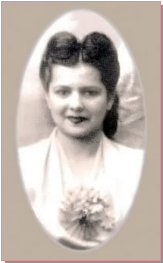
\includegraphics[width = 0.4\linewidth]{4/Tia Mariazinha.png}
\caption{A bela Tia Mariazinha.}
\end{figure}

Um acordo firmado entre marido e mulher vetava a realização de sessões de umbanda na casa. 
Para isso, Tio Ângelo havia concordado com a construção do terreiro, ou do Centro, como a Tia Mariazinha o chamava, num outro local. 
Entretanto, minha doença, ao que parece, forneceu à espevitada mãe-de-santo uma excelente oportunidade de provar a superioridade do poder dos orixás sobre a vã medicina dos civilizados. 
Logo ao chegar, eu tinha sido besuntada com óleos perfumados e metida num camisolão de flanela vermelha para desencorajar os maus espíritos. 
Em seguida, fui engalanada com voltas e voltas de guias de santo coloridas em torno do pescoço. 
Durante todo tempo em que lá estive até receber alta, foi vestida nessa flamejante indumentária que percorri consultórios e hospitais. 
Meus pais ficavam embaraçadíssimos, mas eu me achava linda. 

Como meu tio frequentemente passava noites de plantão na sua casa de saúde em Madureira, minha tia sentiu-se encorajada a ignorar o protocolo firmado com o marido e convocou seu pessoal para uma sessão noturna das importantes ali mesmo, no sagrado recinto do seu lar, já que eu, a paciente, não podia abandonar o repouso para ir ao terreiro. 
E foi desse modo que uma noite, no meio do sono, fui desperta para viver uma experiência inesquecível: no quarto semi-iluminado por velas, uma porção de gente vestida de branco entrava para dançar e cantar ao redor da minha cama, ao som do batuque ritmado dos atabaques. 
Mas o espetáculo maior era ela, minha tia: à frente de todos, numa roupa de alvura deslumbrante, enfeitada de colares, pulseiras e balangandãs, babados e mais babados de renda flutuando em imensa nuvem em torno do corpo, ela girava e sambava soberana, esplêndida Iemanjá! 
Pela primeira vez, vi os cabelos que ela arrumava em grosso rolo sobre a nuca, derramados em cascata negra e brilhante até abaixo da cintura. 
Sobre a cabeça, em equilíbrio milagrosamente inalterado pelos passos da dança, um copo de cristal com conchas e água do mar.
 Nunca mais me passou a vontade de um dia me vestir daquela maneira e dançar como a vi fazer naquela noite, deusa branca do candomblé. 
Dias depois, Tia Mariazinha achou necessário fazer uma nova sessão para reforçar os efeitos da primeira. 
Não vi o que aconteceu. 
A casa era um sobrado sólido, de grossas paredes, e eu já adormecera no andar de cima. 
Mas mamãe contou que meu tio chegou inesperadamente e o ritual foi abortado pela mais fulgurante explosão de ira que ela já tinha presenciado num Filpi. 
Caboclos, exus, babalaôs e babalorixás desceram desabalados rua abaixo. Não sobrou um para contar história. 

Ao fim de três semanas, já operada da garganta, comecei a melhorar e assim que me libertei do repouso, passei a freqüentar a oficina do quintal, onde a tia fazia inacreditáveis e delicadas camélias de veludo e cetim, rosas e violetas de organdi e seda e as arrumava em elegantes arranjos que as senhoras usavam à lapela dos ``tailleurs'', no decote, à cintura dos vestidos ``soirée'', ou ainda sobre a aba dos lindos chapéus que saíam daqueles dedos habilidosos e iam sendo arrumados em caixas sobre um tabuleiro enorme que depois ela punha à cabeça e, com seu displicente gingado de cabrocha, ia entregar nas casas das freguesas.

No aniversário da minha mãe, essa nordestina que jamais usou seu sofisticado bom gosto em favor de si mesma, orientou meu pai a comprar um corte de organza e renda francesas na ``Casa Canadá'', templo da moda carioca de então. 
Dentro da embalagem, sobre o negro transparente dos preciosos tecidos, colocou um ramo de rosas de organdi. 
Nunca vi outro igual. 
Foi o traje mais aristocrático que a minha mãe teve em toda sua vida. 

Uma semana depois, liberada já pelos médicos, preparava\hyp{}me para voltar para casa. Não sem antes conhecer o mar, o Corcovado, subir de bondinho o Pão de Açúcar e tomar sorvete na Confeitaria Colombo. 
Tinha viajado de trem e, suprema ventura, pela segunda vez ia tomar um avião. 
Na vinda tinha sido um Viscount e na volta seria um Constellation. 

Antes de partirmos, Tia Mariazinha exigiu que meu pai enchesse de moedas uma gamela de barro para ser enterrada lá em cima do morro, em sinal de gratidão às entidades às quais, na opinião dela, eu incontestavelmente devia minha cura. 
Por via das dúvidas, ele achou prudente não contrariar. 
E lá foi ela, encosta acima, gamela equilibrada sobre a cabeça, confiante para todo o sempre no poder e na proteção das suas bárbaras divindades. 
Por causa desta fé, quando, muitos anos depois da morte do meu tio, bastante doente e sofrendo dores terríveis, ela permitiu que seu filho finalmente a entregasse aos médicos, já era tarde: um câncer devastador tomara conta do seu corpo e nada mais havia para fazer. 

Ainda hoje são vívidos na minha lembrança a preocupação, a atenção e o carinho beirando a ternura com que os meus tios Ângelo, Zico, Bepe e, principalmente, meu próprio pai, que tinham como denominador comum o gênio tempestuoso e o pavio demasiadamente curto, cuidaram de mim e mantiveram em suspenso suas próprias vidas até me ver restabelecida. 
Como também nunca esqueci as noites em claro da minha mãe à minha cabeceira e seus cuidados incessantes, exclusivos e quase ciumentos, capítulos de um longo aprendizado do exercício da maternidade que ela então começou a me ensinar.

De todo o episódio, restou-me a descoberta de uma veia dramática que eu continuaria a explorar em favor dos meus objetivos, sem nenhum pudor, e um campo maior e mais rico para os meus devaneios de menina.
Eu tinha descoberto um mundo para além das ruas da minha cidade. 
Comecei a me interessar por moda e desenhava mocinhas copiadas das revistas ostentando flores no cabelo, nos vestidos esvoaçantes e nos chapéus.  
E acho que me ficou, lá no fundo, fruto da convivência com a estranha tia macumbeira, sua cobra e seu animismo, uma empatia em estado de dormência que haveria de se manifestar no dia em que, através da leitura de Gabriel Garcia Márquez, fui apresentada ao estilo, às histórias e personagens delirantes dos escritores do realismo mágico latino-americano.

Na fase araraquarense da doença, o sacrifício imposto pelo longo período de repouso atenuou-o a alegre e redonda Ondina, empregada da fábrica do meu pai, que todos chamavam pelo curto e marinho apelido de Onda e que, posta a zelar diariamente para que eu não me agitasse, ensinou-me a fazer roupinhas de boneca. 
Caiu-me tanto no gosto a brincadeira que ainda as fazia, já mulher feita, para vestir as bonecas da Paula.

Acho que se acirrou, também, a partir daí, uma longa relação de rivalidades e atritos que marcaria, por muitos e muitos anos, a convivência entre mim e Reginaldo, meu irmão mais próximo. 
Por cerca de seis meses a família gravitara quase exclusivamente em torno da minha saúde. 
A partida para o Rio de Janeiro fora abrupta e ele, com quatro anos, tinha sido deixado sem maiores explicações aos cuidados do Tio Totó, o irmão do meu pai que morava na fazenda e que, entre todos os Filpi, era o mais rude e severo. Se tivesse nascido nos dias de hoje, creio, meu irmão seria diagnosticado como uma criança hiperativa. 
Era magricela, agitado e provocador. 
Com certeza foi submetido, mais de uma vez, aos duros métodos do Tio Totó. 
O fato é que quando, ao voltar, meus pais foram buscá-lo na fazenda, tiveram que caçá-lo no meio do pasto como a um potro bagual. 
Ele corria e gritava que não era filho deles. 
Até a idade adulta, vez ou outra, entre brincando e sério, ele manteve o estranho hábito de perguntar à minha mãe se não era verdade que fora adotado. 
E, por igual período, pareceu sentir enorme prazer em me atazanar sempre que a ocasião se apresentasse propícia. 

Para finalizar, minha mãe ficou presa de uma ansiedade que ela só conseguia resolver ministrando-me quantidades enormes de mingau de aveia e certificando-se, refeição após refeição, de que eu não deixara sobrar nada no prato. Quatro anos depois, eu me tornara uma criança obesa.

\chapter{}
Minha mãe era professora normalista e começou sua carreira como todas começavam na época, numa escola rural. 
Meu pai nunca aceitou que ela trabalhasse fora de casa, mas, com a ajuda de políticos, mamãe conseguiu que criassem para ela uma vaga na Fazenda Barrinha, que pertencia ao Tio Zé Amaral, marido da Tia Yolanda, irmã mais velha do papai. 
O plano era levar  meu irmão e eu junto com ela, pois o regulamento para ingresso na carreira exigia que ela estagiasse numa escola rural por pelo menos um ano até que fosse possível tentar uma transferência para a cidade. 
Papai permaneceria em casa e nos visitaria nos finais de semana. 
Tudo acertado, com a relutante concordância do marido, mamãe convocou a Vó Didi para providenciar nossos trajes de roça. 
As duas foram para a rua e pouco tempo depois voltaram sobraçando uma peça de brim azul-marinho. 
Rapidamente vovó desmanchou-a e tornou a dobrá-la em pregas largas sobre as quais recortou assim uma espécie de mamulengo com as nossas medidas, meia peça para cada um. 
Isso feito, sentou-se à máquina de costura e, em algumas horas, Reginaldo e eu envergávamos uma versão pioneira do macacão celebrizado, anos mais tarde, pela Revolução Cultural de Mao Tsé-Tung, na China. 
Para completar a elegância, ganhamos dois pares de Alpargatas Roda cada um, uma sapatilha de lona e corda usada pelos trabalhadores da lavoura naquele tempo. 
No dia seguinte, lá fomos nós de mala e cuia para a Barrinha.
                     
A escola era um comprido barracão de madeira apoiado sobre um baldrame de tijolos, para impedir a entrada de cobras. 
Tinha um odor peculiar de que me lembro até hoje, mistura de madeira seca com pó de giz, acrescido do cheiro de picumã que as crianças traziam na roupa por causa da fumaça dos fogões de lenha que as mal ventiladas casas da colônia não conseguiam dispersar. 
Do depósito de selas e tralhas contíguo à sala de aula, vinha se juntar o bodum de couro suado do lombo dos animais. 
Mas a escola, como tudo o que rodeava Tia Yolanda, era limpíssima, lavada e esfregada com soda. Na mesa, um vaso sobre a toalha bordada e engomada com esmero, aguardava o ramalhete improvisado colhido pelos alunos ao longo do caminho.  


\begin{figure}[H]
\centering
\includegraphics[width=0.4\linewidth]{5/mamãe+reginaldo.png}
\caption{Mamãe, Reginaldo e eu diante.}
\end{figure}

\begin{figure}[H]
\centering
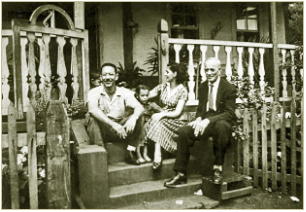
\includegraphics[width=0.6\linewidth]{5/papai+vô joão.png}
\caption{Papai e Vô João nos visitando na sede da fazenda.}
\end{figure}

O primeiro dia de aula numa escola rural tinha que ser invariavelmente dedicado a examinar as unhas, o cabelo e as mãos da criançada.
Piolho, unha suja, pescoço encardido, bicho de pé, nada escapava ao rigoroso escrutínio da brigada sanitária integrada pela minha mãe e pelo casal de tios. 
Na beira do poço, um a um, os alunos iam sendo examinados, lavados e escovados para aprender como deviam se apresentar diante da professora dali em diante. 
Era a primeira lição.

Olhando aqueles meninos atentos e obedientes à minha mãe, que chegavam alegres como uma revoada de andorinhas apesar da dura batalha de todos os dias para vencer os esses e erres, para imitar o talhe impecável da letra da professora, para desvendar os mistérios das divisões e multiplicações, é que eu comecei a achar que essa história de estudo devia ser muito importante mesmo. 
Mas, como esperar que mantivessem os cadernos limpos e organizados como minha mãe queria, se naquele lugar não havia como se livrar da terra nas mãos, nas roupas, na cara, em toda parte? 
Pois não é que eles acabavam conseguindo?  
O ano mal ia a meio e a maioria deles já tinha uma letra redonda e ligeiramente inclinada, como queria a professora, os cadernos encapados, com os parágrafos, margens e vinhetas apropriadamente distribuídos. 
Minha mãe era brava, mas vibrante, entusiasmada e gostava de cantar com eles. 
Também sabia fazer bonitos desenhos na lousa para ilustrar os temas das aulas. Talvez por isso, mais do que atenção, medo ou respeito, o que eu via na expressão daquelas crianças era gratidão, quase adoração.

\begin{figure}[H]
\centering
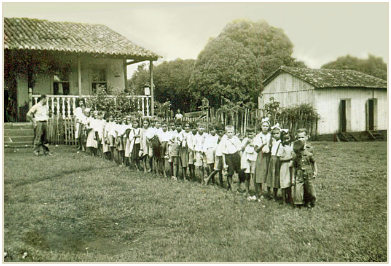
\includegraphics[width=0.6\linewidth]{5/escola.png}
\caption{Os alunos da Fazenda Barrinha, Reginaldo e eu à frente.}
\end{figure}

Foi naquela humilde escolinha rural da Fazenda Barrinha que, sem me dar conta, encantei-me pelo ofício de ensinar.  
E de aprender. 
Era fascinante observar como aquelas crianças, pouco mais que animaizinhos mudos e assustados no primeiro dia de aula, iam se afirmando na sua humanidade, à medida que progrediam nos estudos. 
Pareciam mais alegres, mais confiantes, como se as porteiras do mundo fossem se abrindo diante deles e aquele ingênuo desenho da estrada florida e ensolarada que estampava as capas dos cadernos baratos que o governo lhes fornecia, fosse se materializando diante dos seus olhos.  
Por causa disso, quando eu própria cheguei à idade de frequentar a escola, tinha desse universo a melhor das impressões.
    
A hoje pejorativamente chamada escola reprodutivista, de inspiração cartesiana, tinha o efeito de tornar o mundo muito simples e seguro para as crianças daquele tempo. 
Quem duvidaria que o Brasil fora descoberto por culpa das calmarias na costa africana, se quem o afirmava era Dona Anahyde, minha professora de 4ª série, corpulenta senhora de cabelos vermelhos colados à testa em caprichadas ondinhas e expressão feroz de um guarda penitenciário? 
Aliás, como mamãe proclamava orgulhosamente, fiz meu primário com as melhores professoras do Grupo Escolar, a começar por ela própria, o que significava, principalmente, ter experimentado as mais rígidas disciplinadoras da casa. 
Tenho certeza de que ao cabo da minha vida, a última coisa a se apagar na memória serão os nomes das cidades percorridas pela Estrada de Ferro Central do Brasil, decorados no dia em que Tia Odete, que se gabava de ouvir um alfinete cair na sua silente classe de 3º ano, manteve-me em pé diante do mapa da dita ferrovia durante a tarde toda, porque olhei para trás durante suas explicações, ao ter o cabelo puxado por meu irmão. 
O mundo se dividia, claramente, entre o certo e o errado, o bem e o mal, sem atenuantes, sem nuances, sem relativismos, sem dúvidas. 
Havia uma resposta correta para tudo e a resposta era aquela da professora. 
E os pais estavam de pleno acordo quanto a isso. 
Portanto, podíamos brincar despreocupados no recreio. A vida era previsível e se alguém tivesse cabeça boa para decorar e obedecer a regras e instruções, não havia o que temer. 

Um dia, já Coordenadora Pedagógica de um colégio jesuíta no Piauí, desci aos porões do centenário prédio atrás de livros antigos de aritmética. 
Remexendo as estantes empoeiradas do arquivo, encontrei, caído por detrás delas, um grande caderno de gravuras que o Ministério da Educação distribuía, até meados do século XX, por todas as salas de aula do país e que eu vi, pela primeira vez, na escola da Barrinha.  
Era o material de apoio utilizado nas aulas de redação, numa prática anunciada como ``composição à vista de uma gravura'' e que podia ser, alternadamente, uma descrição ou uma narração. 
Consistia numa sucessão de estampas ingênuas, exibindo crianças e animaizinhos felizes em campos floridos, árvores frondosas, casinhas aninhadas entre montanhas, nuvens brancas e gorduchas por sobre as quais brilhavam invariavelmente os raios amarelos do sol. 
Judiciosamente, a professora dava o começo, escrito em letras caprichadas na lousa: ``Era uma linda manhã de primavera\dots''. 
As reticências eram a deixa para que nós, os alunos, fôssemos em frente. 
Maravilhada, corri para exibir o achado à minha colega de Coordenação, Jovina, que tinha mais ou menos a minha idade e, portanto, devia ter cursado o primário na mesma época.  
Paulista eu, piauiense ela, descobrimos, às gargalhadas, que a distância de alguns milhares de quilômetros não impedira a inacreditável coincidência de adjetivos, advérbios e frases feitas inspiradas pelas tais gravuras e que, usados em profusão, garantiram para ambas a aprovação com louvor naquela matéria. Assim que passou o surto de hilaridade, minha colega comentou: 

{\itshape``-- Hoje a gente ri, mas me diga, aqui na escola, quando é preciso redigir um discurso, um ofício, um requerimento ou até uma simples comunicação, é atrás de nós duas que eles vêm, é, ou não é?''}
\chapter{}
Fui, ao longo da minha vida escolar, uma boa aluna. 
Não porque fosse uma grande estudiosa, mas sim, porque aprendi a gostar de ler. Meu pai tinha o hábito de, logo depois de retirada a louça do jantar, abrir o jornal sobre a mesa e comentar em voz alta as notícias do dia. 
Parecia tirar um grande prazer disso, de tal forma que comecei a encarapitar-me junto dele, querendo partilhar do ritual, embora fosse ainda muito pequena para entender qualquer coisa. Achando graça, papai começou a soletrar comigo o título do jornal até que “Folha da Manhã” foi a primeira coisa que li na vida, com dígrafos, til e tudo. 
Com o passar dos anos, de alguma maneira devo ter percebido que nos livros estavam as respostas para o meu precoce interesse pelas pessoas e pela vida em geral. 
Além disso, logo ficou claro para mim que a leitura proporcionava um agradabilíssimo e rendoso disfarce para a minha dificuldade de memorizar, deficiência preocupante na vigência de uma prática escolar em que a promoção dependia exclusivamente do talento do aluno para reproduzir com absoluta fidelidade o que ensinavam os livros ou o professor. 
Descobri que só guardava o que conseguia entender, digerir e devolver com minhas próprias palavras e a leitura foi a grande responsável pela facilidade com que passei a realizar tais operações. 

Acho que o ponto alto da minha estratégia para ocultar dos professores a incapacidade de decorar aconteceu quando eu cursava a oitava série, no dia em que a mais temida professora do Colégio, D. Cidinha, professora de História, chamou-me para entregar uma prova e perscrutando-me miudamente o rosto, disse:
 
{\itshape``-Teresa, dei-lhe uma nota oito, porque sua narração da revolta pela libertação da Grécia não só está bem redigida, como satisfatoriamente fiel; entretanto, como você omitiu datas e nomes, é verdade que ela se ajustaria à maior parte das revoluções da História. Na pior das hipóteses, você parece ter aprendido bastante sobre a dinâmica dos movimentos revolucionários.''}

Lembrei-me deste fato quando me tornei eu própria uma professora de História e passei a inaugurar meus cursos comunicando aos espantados alunos que naquele ano experimentariam uma novidade: uma professora de História desmemoriada, incapaz de guardar datas e nomes, mas muito interessada nos porquês da História e, principalmente no uso que poderíamos fazer deles para as nossas vidas. 

Mas, ai de mim, nas então pretensiosamente chamadas “ciências exatas”, com relevo especial para a Matemática, nenhuma estratégia funcionava. 
Tudo me parecia de um autoritarismo monolítico, intolerável, com suas regras, axiomas e princípios. 
Enquanto estudei aritmética saí-me até bem, pois, como lembrou um nosso cronista, acho que Rubem Braga, havia enredo na coisa. 
Havia ética que convidava à solidariedade no esforço de encontrar o troco exato ou de repartir terrenos, laranjas ou bolas de gude de modo que o resultado fosse perfeitamente aceitável para os interessados. 
Quando, porém, ao ingressar no ginásio, fui conduzida por aquele que seria meu único professor da matéria a partir daí, aos tenebrosos domínios da Álgebra, uma parte do meu cérebro entrou em colapso e pareceu soçobrar no oceano escuro da ignorância. 
Para sempre. 
Tornei-me, desde então, incapaz de pensar a vida em números. 
Avessa a medir e contar, fosse lá o que fosse. Mistério considerado insondável por quantos se detiveram a analisar o problema. 

Aquele professor era proclamado um gênio por toda a cidade. 
Muito magro e agitado, avental imaculadamente branco, cheirando a lavanda e cigarro, ele entrava na classe já ditando a lição e escrevendo compulsivamente no quadro negro. Como hieróglifos numa tumba egípcia, intermináveis equações, trinômios, polinômios iam se estampando em ritmo frenético por toda a lousa e, quando esta se esgotava, pelas paredes. 
O giz ia se despedaçando entre os dedos nervosos e espalhando-se pelo chão. 
A intervalos, ele catava os toquinhos e despejava-os numa caixa. 
Tinha uso para eles: atirava-os na cabeça dos distraídos. 
Eu estava entre os seus alvos preferidos. Ao lado da escola, uma imensa paineira lançava ao vento delicados flocos que entravam pela janela da sala e flutuavam como bailarinas minúsculas diante dos meus olhos enlevados.  
Desse devaneio me tirava a voz aguda do professor e o concomitante estalinho do toco de giz sobre a testa:

{\itshape“- {\large\bfseries D o n a T e r e s a F i l p i}, depois não sabe por que não entende   Matemática, não é?”}

Por vias indiretas, devo muito a esse professor. 
Não sei por que, encasquetei com a idéia de encaminhar-me para Medicina quando cheguei ao curso médio ou Colegial, como era chamado então. 
Para tanto, matriculei-me no Científico, opção que enfatizava as Ciências Exatas, com aulas diárias e reforçadas de Matemática. 
Ao dar comigo na classe de primeiro ano, um esgazeado Sr. Ulysses, era assim que ele se chamava, abandonou a sala e dirigindo-se a um telefone ligou para minha mãe exigindo que ela providenciasse a minha imediata transferência para o curso Clássico, que preparava para as faculdades de Línguas e Ciências Humanas. 
Minha mãe obedeceu no ato. Odiei-o por isso e por muito tempo julguei-me frustrada em minha vocação. 
Tornei-me então, educadora. 
Muito tempo depois, haveria de ter um contato mais próximo com a vida de um médico quando, durante a recuperação de uma fratura no pé, trabalhei com meu irmão João na sua clínica de ortopedia. 
Só então é que, no íntimo, agradeci fervorosamente àquele impaciente professor. Jamais teria experimentado pela rotina médica a paixão que me despertou a batalha diária nas salas de aula. 
E mais, a lembrança do martírio que esse professor e eu mutuamente nos infligimos, me orientou a empreender uma revolução no ensino de Matemática do colégio que eu coordenei. 
Jamais consegui aceitar que uma ciência que nasceu para favorecer a harmonia e a ética, educando os homens para a honestidade e para a civilidade, fosse tão desvirtuada por uma pedagogia arbitrária e pretensamente neutra, a pretexto de ser “científica”. 

A baixa remuneração dos professores, uma triste recorrência na história da educação brasileira, sempre trouxe como efeito, entre tantos outros, a absurda carga horária assumida pela maioria deles e que fazia com que, à semelhança do que me ocorreu com a Matemática, os alunos, numa determinada disciplina, tivessem o mesmo professor por anos a fio. 
Havia deles que ministravam aulas desde o início do primeiro grau até o fim do segundo. 
Quando eram bons, isto era uma sorte incrível na mediocridade reinante. 
Mas, se eram deficientes, o aluno ficava lesado para todo o sempre. 
Aconteceu-me com Geografia, além de Matemática. Ainda hoje ostento uma dificuldade irritante, verdadeiramente limítrofe, para me orientar no espaço. 
Mas, em Português, em compensação, tive, por seis anos consecutivos, um professor maravilhoso que se sustentara na faculdade interpretando radionovelas e que adorava ler para nós. 
Aprendi a língua como quem aprendesse música. 
Nunca soube, como continuo a não saber, regras gramaticais, porque ele não nos aborrecia com isso. 
Aprendi a escrever lendo com ele gente que escrevia bem.  
E ouvindo aquela voz sonora e expressiva realçando o estilo e a elegância do autor. 
Meu velho e querido Professor Jurandyr. Muito aprendi também com Dona Elisa, sobrinha de Mario de Andrade, por curtos anos minha professora de francês e que falava de autores e livros como quem descrevesse delícias culinárias. 
Salivando gulosamente. 
E provocando, em quem a ouvia, uma fome danada de ler. 
E Dona Olga, poetisa de parnasianos versos, uma típica sobrevivente de tempos machadianos, cujo pai tinha sido amigo muito chegado de Ruy Barbosa. 
Anacrônica dama, capaz de exigir dos seus aluninhos, como lição de casa, doze sinônimos para o adjetivo cinzento. 
Que Deus abençoe a todos, quanto lhes devo!

\end{document}